% Options for packages loaded elsewhere
\PassOptionsToPackage{unicode}{hyperref}
\PassOptionsToPackage{hyphens}{url}
\documentclass[
  10pt,
  conference]{IEEEtran}
\usepackage{xcolor}
\usepackage[margin=1in]{geometry}
\usepackage{amsmath,amssymb}
\setcounter{secnumdepth}{-\maxdimen} % remove section numbering
\usepackage{iftex}
\ifPDFTeX
  \usepackage[T1]{fontenc}
  \usepackage[utf8]{inputenc}
  \usepackage{textcomp} % provide euro and other symbols
\else % if luatex or xetex
  \usepackage{unicode-math} % this also loads fontspec
  \defaultfontfeatures{Scale=MatchLowercase}
  \defaultfontfeatures[\rmfamily]{Ligatures=TeX,Scale=1}
\fi
\usepackage{lmodern}
\ifPDFTeX\else
  % xetex/luatex font selection
\fi
% Use upquote if available, for straight quotes in verbatim environments
\usepackage{bookmark}
\IfFileExists{xurl.sty}{\usepackage{xurl}}{} % add URL line breaks if available
\urlstyle{same}
\hypersetup{
  hidelinks,
  pdfcreator={LaTeX via pandoc}}

\title{Continuous Deployment as Cost-Sensitive Decision-Making:\\
When Contextual Bandits Outperform Static Rules and When They Don't}

\author{%
  \IEEEauthorblockN{Abishek Kumar Giri}
  \IEEEauthorblockA{%
    Stockton University\\
    giriabishekkumar5@gmail.com\\
    ORCID: 0009-0005-9082-9887
  }
}

\date{}

% figure + table packages
\usepackage{graphicx}
\usepackage{booktabs,array,multirow}
\providecommand{\tightlist}{\setlength{\itemsep}{0pt}\setlength{\parskip}{0pt}}

% float-packing tuning (typography only)
\renewcommand{\topfraction}{0.9}
\renewcommand{\bottomfraction}{0.9}
\renewcommand{\textfraction}{0.1}
\renewcommand{\floatpagefraction}{0.75}
\setlength{\floatsep}{6pt plus 2pt minus 2pt}
\setlength{\textfloatsep}{8pt plus 2pt minus 2pt}
\setlength{\intextsep}{6pt plus 2pt minus 2pt}

% pandoc code-highlighting environments
\usepackage{fancyvrb}
\usepackage{framed}
\newenvironment{Shaded}{\begin{framed}}{\end{framed}}
\DefineVerbatimEnvironment{Highlighting}{Verbatim}{commandchars=\\\{\}}
\newcommand{\KeywordTok}[1]{\textbf{#1}}
\newcommand{\StringTok}[1]{#1}
\newcommand{\CommentTok}[1]{\textit{#1}}
\newcommand{\OtherTok}[1]{#1}
\newcommand{\NormalTok}[1]{#1}
\newcommand{\DataTypeTok}[1]{#1}
\newcommand{\DecValTok}[1]{#1}
\newcommand{\BaseNTok}[1]{#1}
\newcommand{\FloatTok}[1]{#1}
\newcommand{\ConstantTok}[1]{#1}
\newcommand{\CharTok}[1]{#1}
\newcommand{\SpecialCharTok}[1]{#1}
\newcommand{\VerbatimStringTok}[1]{#1}
\newcommand{\SpecialStringTok}[1]{#1}
\newcommand{\ImportTok}[1]{#1}
\newcommand{\DocumentationTok}[1]{\textit{#1}}
\newcommand{\AnnotationTok}[1]{\textit{#1}}
\newcommand{\CommentVarTok}[1]{\textit{#1}}
\newcommand{\VariableTok}[1]{#1}
\newcommand{\ControlFlowTok}[1]{\textbf{#1}}
\newcommand{\OperatorTok}[1]{#1}
\newcommand{\BuiltInTok}[1]{#1}
\newcommand{\ExtensionTok}[1]{#1}
\newcommand{\PreprocessorTok}[1]{#1}
\newcommand{\AttributeTok}[1]{#1}
\newcommand{\RegionMarkerTok}[1]{#1}
\newcommand{\InformationTok}[1]{\textit{#1}}
\newcommand{\WarningTok}[1]{\textbf{\textit{#1}}}
\newcommand{\AlertTok}[1]{\textbf{#1}}
\newcommand{\ErrorTok}[1]{\textbf{#1}}
\newcommand{\FunctionTok}[1]{#1}

\begin{document}

\maketitle

\begin{center}\rule{0.5\linewidth}{0.5pt}\end{center}

\section{Abstract}\label{abstract}

Continuous deployment pipelines make deployment decisions millions of
times per day across the industry, yet whether to treat them as
classification or as sequential cost minimization has not been
empirically settled. This paper characterizes the operating envelope of
contextual-bandit deployment control: the cost-asymmetry, failure-rate,
and trajectory-length conditions under which adaptive policies
outperform static rules, and the conditions under which they do not. We
apply disjoint LinUCB (Li et al., 2010) and Bayesian linear Thompson
Sampling (Agrawal \& Goyal, 2013) to the three-action problem \{deploy,
canary, block\} with an asymmetric cost matrix and a pending-reward
buffer enforcing the delayed-feedback invariant.

The strongest result is the cost-ratio sweep: the bandit advantage over
a static rule scales monotonically from -7\% at 5:1 to -49.6\% at 100:1.
The default 20:1 ratio sits precisely at break-even; the case for
adaptive control is material only above 40:1. Within the bandit family,
Thompson Sampling outperforms LinUCB by 6.8\% on real GitHub Actions CI
data (Thompson 624 vs.~LinUCB 669.5; bootstrap 95\% CI {[}598, 648{]}
entirely below LinUCB mean, p \textless{} 0.0001 over 10,000 resamples).
The static-rule cost (644.5) falls inside Thompson's CI --- the two are
statistically tied. In this regime, the exploration-strategy choice
matters more than the bandit-vs-rule choice.

The envelope has a hard lower boundary. On real GitHub Actions data (600
runs, two public repositories) with a 5.3\% failure rate and no
commit-level features, LinUCB over-blocks and costs 3.8\% more than a
static rule; 300-step trajectories leave the policy below the O(d$^{2}$) =
169 updates-per-arm convergence threshold. Drift adaptation via
PageHinkley detection is net-negative across all three drift modes ---
stationary, abrupt, and gradual --- due to false-alarm resets at the
default sensitivity ($\lambda$ = 50), firing 10.6 resets per trajectory on
stationary data. The bandit framing adds genuine value by making cost
assumptions explicit and treating the canary decision as a first-class
action; the algorithmic gains over static rules are conditional on
operating above the envelope boundary.

\begin{center}\rule{0.5\linewidth}{0.5pt}\end{center}

\section{1. Introduction}\label{introduction}

\subsection{1.1 The Deployment Decision
Problem}\label{the-deployment-decision-problem}

Every passing continuous integration (CI) build triggers a deployment
decision: ship to production, route through a canary, or block? A failed
production deployment means incidents, on-call pages, and rollbacks. A
blocked safe change costs developer time. A canary offers partial
protection at throughput cost. Getting this right matters, and at scale
it happens thousands of times per day.

Current tooling treats this as a prediction problem. Just-in-time defect
prediction models (Kamei et al., 2013; McIntosh \& Kamei, 2018) estimate
failure probability and apply a static threshold. Three structural
limitations follow:

\begin{enumerate}
\def\labelenumi{\arabic{enumi}.}
\tightlist
\item
  \textbf{The threshold encodes an implicit cost assumption.} Setting it
  requires a judgment about the cost of blocking safe changes
  vs.~deploying bad ones. This assumption is rarely explicit and never
  adapts.
\item
  \textbf{Costs are asymmetric and context-dependent.} A production
  incident at a payment service costs an order of magnitude more than
  one at an internal tool. A single fixed threshold cannot represent
  this.
\item
  \textbf{The model does not learn from outcomes.} JIT models are
  trained offline on defect labels. They receive no feedback when
  predictions lead to incidents or unnecessary blocks.
\end{enumerate}

\subsection{1.2 Our Framing: Sequential Cost
Minimization}\label{our-framing-sequential-cost-minimization}

We model deployment control as a \textbf{contextual bandit}: at each
decision step \emph{t}, the controller observes a context vector
\emph{x\_t} (commit metadata, CI signal, change type, author history)
and selects an action \emph{a\_t} $\in$ \{deploy, canary, block\}. A reward
\emph{r\_\{t+k\_t\} = -cost(a\_t, outcome\_\{t+k\_t\})} arrives
\emph{k\_t} steps later, where \emph{k\_t} reflects the time until the
deployment outcome is observable.

This framing differs from classification in three ways:

\begin{itemize}
\tightlist
\item
  \textbf{The objective is cumulative cost minimization, not accuracy
  maximization.} The policy is evaluated on what it costs to act, not on
  whether it correctly predicts a label.
\item
  \textbf{The three-action space makes the canary option a first-class
  decision.} We model the action directly rather than applying a
  threshold to a risk score.
\item
  \textbf{The policy learns online from its own decisions.} Each
  deployment outcome updates the policy's belief about which actions are
  cost-effective in which contexts.
\end{itemize}

\subsection{1.3 When Does the Bandit Framing Pay
Off?}\label{when-does-the-bandit-framing-pay-off}

The bandit advantage is not unconditional. Two conditions must hold
simultaneously for a contextual bandit to outperform a well-tuned static
rule:

\textbf{Condition 1 --- sufficient failure rate asymmetry.} When failure
rates are very low (say, 5\%), the deploy arm is nearly always optimal
regardless of context. A static rule that deploys aggressively matches
the oracle. A bandit with exploration budget $\alpha$ wastes decisions sampling
suboptimal arms (canary, block) before its posterior converges. The
exploration cost dominates the expected gain.

\textbf{Condition 2 --- sufficient informative context.} LinUCB with a
\emph{d}-dimensional feature vector needs roughly \emph{O(d$^{2}$)} updates
per arm before its parameter estimates are statistically meaningful.
With \emph{d} = 13 in our setup, that is approximately 169 updates per
arm before the confidence interval shrinks to first-order accuracy. On a
300-step real-world trajectory, the bandit has barely enough data to
form reliable per-arm estimates, let alone differentiate arms based on
context. If the feature vector carries no commit-level signal (no files
changed, no test counts), the bandit degenerates to learning from
failure rate and a bias term --- information a static rule can encode
directly.

When both conditions fail --- low failure rate, feature sparsity, short
trajectory --- static rules are competitive and bandits may be worse.
This paper documents both regimes empirically.

Beyond the two conditions, our experiments surface an orthogonal
limitation of posterior sampling: even after convergence (200 updates
per arm for smoke/alpha, 183 for smoke/beta, both above the O(d$^{2}$)=169
threshold), Thompson Sampling's posterior never collapses to the optimal
arm. Thompson persistently allocates 22.4\% to canary at a failure rate
where block is cheaper, while LinUCB's upper confidence bound (UCB)
criterion concentrates on the highest-confidence arm and reaches 86.3\%
block. Posterior variance, not sample size, is the driver. We discuss
this in §5.1.

\subsection{1.4 Contribution Summary}\label{contribution-summary}

LinUCB and Thompson Sampling are well-established algorithms. Our
contributions are in problem framing and empirical characterization:

\begin{itemize}
\tightlist
\item
  \textbf{Reframing:} Deployment control recast as sequential cost
  minimization with a three-action space \{deploy, canary, block\} and
  an explicit asymmetric cost matrix. Cumulative cost replaces accuracy
  as the primary metric.
\item
  \textbf{Evaluation framework:} Online-replay protocol with a
  pending-reward buffer enforcing the delayed-feedback invariant;
  explicit bias disclosure; cost as the sole headline metric.
\item
  \textbf{Component ablation:} Cost weighting, delayed feedback, and
  drift adaptation isolated and quantified. Cost weighting is the
  dominant factor (+31\% cumulative cost when removed); drift
  adaptation, under the chosen Page-Hinkley calibration, is net-negative
  across all three drift modes due to false-alarm resets --- a measured
  limit of off-the-shelf drift detectors on cost-stream data.
\item
  \textbf{Two-sided empirical characterization:} Bandits outperform
  static rules on the synthetic environment used in this study when
  failure costs are high and context is informative.
  In the low-failure regime with feature sparsity (5.3\% failure rate,
  no commit-level features), UCB-based policies over-block and cost
  3.8\% more than a static rule --- a negative result that defines the
  operating envelope of the framing. A cost-ratio sweep (5:1 to 100:1)
  confirms the advantage is monotone: the default 20:1 ratio in this
  paper sits at the envelope boundary where bandits break even; at 40:1
  and above, the advantage is 19--50\%.
\item
  \textbf{Within-bandits exploration finding:} In the feature-sparse
  regime where LinUCB underperforms, Thompson Sampling outperforms
  LinUCB by 6.8\% on real data (CI {[}598, 648{]} entirely below LinUCB
  = 669.5; p \textless{} 0.01). Thompson and the static rule are
  statistically tied. The choice of exploration strategy --- posterior
  sampling vs.~UCB --- is the first-order variable in this regime, not
  the bandit framing itself.
\end{itemize}

\subsection{1.5 Related Work}\label{related-work}

\textbf{Just-in-time defect prediction.} Kamei et al.~(2013) establish
the empirical foundation for commit-level defect prediction, training
logistic regression models on change metrics (churn, complexity,
developer experience) across 10,000+ commits from six large open-source
projects. They demonstrate that commit-level features predict defect
introduction with AUC above 0.70 and that developer experience is among
the most informative features. What they do not model: the asymmetric
operational cost of prediction errors, the adaptive adjustment of
thresholds to project-specific failure distributions, or the three-way
deploy/canary/block action space. McIntosh \& Kamei (2018) show that
fix-inducing changes are a moving target --- the feature importance and
model accuracy of JIT prediction shift substantially across time periods
--- motivating approaches that adapt online rather than training a fixed
offline model.

\textbf{Contextual bandits.} Li et al.~(2010) formulate personalized
news recommendation as a contextual bandit problem and introduce LinUCB,
demonstrating that upper-confidence-bound policies using linear payoff
models outperform static and context-free baselines in online A/B
comparisons. They do not address asymmetric costs, delayed rewards, or
three-way action spaces. Chu et al.~(2011) provide theoretical regret
analysis for linear contextual bandits, establishing that the cumulative
regret of LinUCB scales as O($\sqrt{}$(dT log T)) where d is the feature
dimension and T is the horizon; this bound underlies the O(d$^{2}$)
convergence threshold used in §1.3.

\textbf{Evaluation under partial feedback.} Joachims et al.~(2018)
address learning from logged bandit feedback, where only the reward for
the chosen action is observed. They introduce propensity-weighted
empirical risk minimization to debias learning from such data and show
that naive learning from logged feedback produces systematically biased
models. Their analysis is relevant to the online replay evaluation used
here: because every logged action in the TravisTorrent data is DEPLOY,
inverse propensity scoring cannot be applied (log propensity is
identically 1.0), and the bias they identify is present in our results
without correction. We disclose this explicitly in §7.1.

\textbf{Concept drift.} Gama et al.~(2014) survey concept drift
adaptation algorithms for data streams, covering drift detectors,
ensemble methods, and sliding-window retraining. They characterize the
trade-off between detection speed and false-alarm rate that motivates
threshold calibration --- the same trade-off that produces the
false-alarm problem in §6.4. Bifet \& Gavald{\`a} (2007) introduce ADWIN, an
adaptive windowing algorithm that detects changes in the mean of a
stream statistic by testing whether older and newer subwindows have
significantly different distributions. ADWIN provides theoretical
false-alarm and detection-delay guarantees that Page-Hinkley lacks; it
is implemented in this codebase but excluded from the reported
experiments because it was not evaluated on the cost streams used here.

\textbf{Delayed feedback in bandits.} Vernade et al.~(2017) study the
stochastic bandit problem where rewards arrive after a random delay and
may be censored (never arrive). They show that naive algorithms ignoring
delay structure suffer avoidable regret, and they propose algorithms
with regret bounds that account for delay distribution. Their setting
maps directly to the deployment evaluation problem: a CI run takes
minutes to hours, and its deployment outcome (incident or not) may not
be observable within the evaluation window. Joulani et al.~(2013)
address the same delayed-feedback setting for general online learning,
showing that the regret cost of delay is O($\sqrt{}$(d\_max $\cdot$ T)) where d\_max
is the maximum delay. Pike-Burke et al.~(2018) extend delay analysis to
aggregated anonymous feedback. This paper applies the pending-reward
buffer approach from Joulani et al.~(2013) to the deployment context,
routing all policy updates through a buffer that enforces the
delayed-feedback invariant.

\begin{center}\rule{0.5\linewidth}{0.5pt}\end{center}

\section{2. Problem Formulation}\label{problem-formulation}

\subsection{2.1 Contextual Bandit with Delayed
Rewards}\label{contextual-bandit-with-delayed-rewards}

Let \emph{X} be the space of pre-action observable features, \emph{A} =
\{deploy, canary, block\}, and \emph{O} = \{success, failure, censored,
blocked\} the outcome space.

At step \emph{t} the agent observes \emph{x\_t $\in$ X}, selects \emph{a\_t
$\in$ A}, and receives a reward

\begin{verbatim}
r_{t+k_t} = -cost(a_t, outcome_{t+k_t})
\end{verbatim}

after a delay of \emph{k\_t} steps. In our experiments, \emph{k\_t =
max(1, $\lceil$duration\_t / 60$\rceil$)} steps, where \emph{duration\_t} is the build
duration in seconds. The pending-reward buffer holds the reward until
step \emph{t + k\_t}; the policy has no information about it before that
step.

When the outcome is not yet resolved by step \emph{t + max\_delay}, the
reward is \textbf{censored} and excluded from policy updates.

\subsection{2.2 Context Features}\label{context-features}

The feature vector \emph{x\_t $\in$ $\mathbb{R}$\^{}13} encodes 12 pre-action
observables (normalised) plus a bias term:

The 13-dimensional context vector encodes commit-size features (files\_changed, lines\_added, lines\_deleted, src\_churn), CI signal (tests\_run, tests\_added, build\_duration\_s, is\_pr), change-type features (has\_dependency\_change, has\_risky\_path\_change), author/history features (author\_experience, recent\_failure\_rate), and a bias term. Full normalizations are in supplementary Table S1.


All features are available before the deployment action. No post-deploy
signal or outcome appears in \emph{x\_t}.

\subsection{2.3 Cost Matrix}\label{cost-matrix}

The cost function \emph{cost: A $\times$ O $\rightarrow$ $\mathbb{R}$$\geq$0} encodes operational
priorities:

\begin{table*}[t]\centering\footnotesize\begin{tabular}{llll}
\toprule\noalign{}
Action & Outcome & Cost & Interpretation \\
\midrule\noalign{}
\bottomrule\noalign{}
deploy & success & 0.0 & Successful rollout --- no cost \\
deploy & failure & 10.0 & Production incident; on-call, rollback \\
canary & success & 1.0 & Canary overhead + promotion latency \\
canary & failure & 4.0 & Partial-rollout incident, limited blast \\
block & would succeed & 2.0 & Safe change delayed; developer wait \\
block & would fail & 0.5 & Risky change correctly held back \\
block & unknown & 2.0 & Counterfactual unobserved (replay) \\
\end{tabular}\end{table*}

Cost asymmetry is deliberate: deploy + failure (10) is 20$\times$ block +
would\_fail (0.5). Reward is \emph{r = -cost}. The cost matrix is
configurable; §4.3 sweeps it.

\subsection{2.4 Objective}\label{objective}

The policy \emph{$\pi$: X $\rightarrow$ A} minimizes cumulative operational cost over
\emph{T} decisions:

\begin{verbatim}
J($\pi$) = $\Sigma$_{t=1}^{T} cost(a_t, outcome_{t+k_t})
\end{verbatim}

Cumulative operational cost is the sole primary metric throughout this
paper. Action distributions (deploy\%, canary\%, block\%) are reported
as diagnostics to explain \emph{why} a cost difference arose.

\begin{center}\rule{0.5\linewidth}{0.5pt}\end{center}

\section{3. Method}\label{method}

\subsection{3.1 LinUCBWithDrift (Disjoint LinUCB with Cost-Sensitive
Reward and Optional Drift
Reset)}\label{linucbwithdrift-disjoint-linucb-with-cost-sensitive-reward-and-optional-drift-reset}

\texttt{LinUCBWithDrift} applies disjoint LinUCB (Li et al., 2010; Chu
et al., 2011) to the deployment decision, replacing click-through reward
with negative operational cost and routing all updates through the
delayed-feedback buffer. Its update equations are identical to plain
LinUCB; the only structural addition is an optional PageHinkley detector
that can reset the per-arm weight matrices on drift events.

\textbf{Per-arm model.} For each arm \emph{a $\in$ A}:

\begin{verbatim}
A_a $\in$ $\mathbb{R}$^{d$\times$d},  initialized to $\lambda$I
b_a $\in$ $\mathbb{R}$^d,       initialized to 0
$\theta$_a = A_a^{-1} b_a
\end{verbatim}

\textbf{Action selection:}

\begin{verbatim}
UCB(a) = $\theta$_a^T x_t + $\alpha$ $\sqrt{}$(x_t^T A_a^{-1} x_t)
a_t    = argmax_{a $\in$ A} UCB(a)
\end{verbatim}

\textbf{Update rule} (on matured reward \emph{(x\_i, a\_i, r\_i)}):

\begin{verbatim}
A_{a_i} $\leftarrow$ A_{a_i} + x_i x_i^T
b_{a_i} $\leftarrow$ b_{a_i} + r_i x_i,  where  r_i = -cost_i
\end{verbatim}

The negative cost signal means the policy learns to prefer arms with
lower expected operational cost.

\subsection{3.2 Thompson Sampling
Baseline}\label{thompson-sampling-baseline}

Bayesian linear Thompson Sampling (Agrawal \& Goyal, 2013) maintains a
per-arm Gaussian posterior over weight vectors:

\begin{verbatim}
Prior:     $\theta$_a ~ N(0, v$_{0}$ $\cdot$ I)
Posterior: $\Lambda$_a = (1/v$_{0}$)I + (1/$\sigma$$^{2}$)$\Sigma$ x$_{i}$x$_{i}$$^{\top}$
           b_a = (1/$\sigma$$^{2}$) $\Sigma$ r$_{i}$ x$_{i}$
           $\mu$_a = $\Lambda$_a^{-1} b_a
\end{verbatim}

Action selection samples \emph{$\theta$\_a \textasciitilde{} N($\mu$\_a,
$\Lambda$\_a\^{}\{-1\})} via Cholesky decomposition and picks \emph{argmax\_a
$\theta$\_a$^{\top}$ x\_t}. Exploration is implicit; no $\alpha$ parameter is needed. Default
hyperparameters: \emph{v$_{0}$ = 1.0}, \emph{$\sigma$$^{2}$ = 0.1}. Updates use the same
negative-cost reward as \texttt{CostSensitiveBandit}.

Thompson's stochastic action selection produces nonzero seed variance:
identical data yields different trajectories across seeds. This makes it
the only policy for which bootstrap CIs are informative in our current
experiment setup (all other policies are deterministic given the same
delayed-feedback schedule).

\subsection{3.3 Delayed Reward Buffer}\label{delayed-reward-buffer}

The \texttt{PendingRewardBuffer} (\texttt{delayed/buffer.py}) holds
\emph{(context, action, cost, outcome, censored)} until
\texttt{pop\_available(t\ +\ k\_t)} is called. No model update occurs
before maturity.

\textbf{The buffer's value is correctness, not performance.} Removing it
improves cost by 1.1\% (§5.3) because immediate feedback accelerates
convergence. The buffer exists to prevent a policy from using future
information at decision time --- a requirement for valid evaluation in
any real deployment setting.

\subsection{3.4 Drift Adaptation (Exploratory --- Excluded from Main
Claims)}\label{drift-adaptation-exploratory-excluded-from-main-claims}

\texttt{CostSensitiveBandit} optionally accepts a Page-Hinkley detector
(Mouss et al., 2004) that triggers model reset on detected distribution
shift (Gama et al., 2014). On stationary data, the detector at
\emph{$\lambda$\_PH = 50} fires 44 false alarms over 1,150 steps, making the
full model 27\% more expensive than the no-drift variant. Drift results
are excluded from main claims; the threshold requires calibration
against non-stationary data not yet available.

\subsection{3.5 Baselines}\label{baselines}

Policy specifications are in supplementary Table S2.


At identical $\alpha$, $\lambda$, and reward signal, \texttt{linucb} and
\texttt{cost\_sensitive\_bandit} are mathematically identical ($\|$b-vector
difference$\|$$_{2}$ = 0 confirmed experimentally). They are reported together
in the main table.

\begin{center}\rule{0.5\linewidth}{0.5pt}\end{center}

\section{4. Experiments}\label{experiments}

\subsection{4.1 Synthetic Dataset}\label{synthetic-dataset}

The primary experiment uses a synthetic dataset
(\texttt{data/raw/travistorrent\_smoke.csv}) generated to match the
TravisTorrent schema (Beller et al., 2017): two projects ---
\texttt{smoke/alpha} (600 builds, 15\% failure) and \texttt{smoke/beta}
(550 builds, 35\% failure), each spanning \textgreater365 days. Full
statistics are in supplementary Table S3. Fixed failure rates and a
deterministic delay model mean bootstrap CIs collapse to zero for all
deterministic policies (Thompson Sampling alone has nonzero seed
variance); no cross-project generalization is possible from this
dataset.

\subsection{4.2 Online Replay Setup and
Bias}\label{online-replay-setup-and-bias}

We use online replay (\texttt{evaluation/online\_replay.py}): the four
policies --- \texttt{static\_rules}, \texttt{heuristic\_score}, LinUCB
(UCB exploration), and Thompson Sampling (posterior sampling), specified
in §3.5 --- learn during trajectory traversal. Costs are \emph{cost(policy\_action,
logged\_CI\_outcome)}, using CI outcome as a counterfactual proxy for
the deployment outcome.

\textbf{Online replay is a biased evaluation.} Every logged action is
DEPLOY (the loader hardcodes this). Costs for CANARY and BLOCK are
counterfactual: we assume CI outcome would be the same regardless of
deployment action. This is approximately valid for TravisTorrent (CI
runs before any deployment) but unverifiable in general. We use online
replay exclusively for learning-dynamics verification, not causal cost
estimation.

\textbf{Configuration (synthetic experiment):}

We use $\alpha$ = 1.0, $\lambda$ = 1.0, Thompson priors $v_0$ = 1.0 and $\sigma^2$ = 0.1, the deterministic delay model $k_t = \max(1, \lceil \text{build\_duration\_s} / 60 \rceil)$, the default cost matrix from §2.3, and seeds 0--29. Full hyperparameters are in supplementary Table S4.


\subsection{4.3 Robustness Conditions}\label{robustness-conditions}

Five conditions test whether conclusions depend on cost matrix or delay
setting: default; high failure (deploy\_failure 10$\rightarrow$20,
canary\_failure 4$\rightarrow$8); low block (block\_safe and
block\_unknown 2$\rightarrow$1); short delay (delay\_step\_seconds
60$\rightarrow$120); long delay (60$\rightarrow$30). Full specifications
are in supplementary Table S5. Percentile bootstrap CI: 10,000
resamples, seed 42, over seeds 0--4.

\subsection{4.4 Ablation Conditions}\label{ablation-conditions}

Four variants isolate each component: \texttt{no\_drift} (reference, no
drift reset); \texttt{no\_delay} (immediate updates, no buffer);
\texttt{no\_cost} (binary reward $-$1/0 instead of $-$cost); \texttt{full}
(+ PageHinkley drift reset). Full specifications are in supplementary
Table S6.


\subsection{4.5 Real-World Sanity Check
Dataset}\label{real-world-sanity-check-dataset}

To test whether the synthetic findings are contradicted by real CI data,
we collected GitHub Actions workflow run history from two public
repositories via the GitHub REST API:

Real dataset statistics are in supplementary Table S7.


\textbf{Schema mapping:} \texttt{head\_sha} $\rightarrow$
\texttt{git\_trigger\_commit}, \texttt{conclusion} $\rightarrow$
\texttt{tr\_status}, timestamps $\rightarrow$ duration. No commit-level features are
available without additional per-commit API calls; fields default to 0.
The feature vector is dominated by the bias term and recent-failure-rate
--- 11 of 13 dimensions carry no project-specific signal.

\textbf{Filter relaxation:} Standard filters (\texttt{min\_builds=500},
\texttt{min\_history\_days=365}) cannot be satisfied by a 20--99 day API
sample. Relaxed to \texttt{min\_builds=100},
\texttt{min\_history\_days=0}. Results are not directly comparable to
the synthetic conditions.

\textbf{Censored rewards:} Cancelled CI runs ($\approx$3\%) produce genuine
censored rewards --- the first experiment confirming real-world
censoring rather than theoretical.

\begin{center}\rule{0.5\linewidth}{0.5pt}\end{center}

\section{5. Results}\label{results}

\subsection{5.1 Main Results (Synthetic
Data)}\label{main-results-synthetic-data}

\textbf{{[}Preliminary --- synthetic 2-project dataset. Deterministic
policies have zero CI width.{]}}

Thompson's higher cost and wider spread relative to LinUCB and static rules are visible; the per-seed distribution is shown in the supplementary material.

\begin{figure}[tbp]
  \centering
  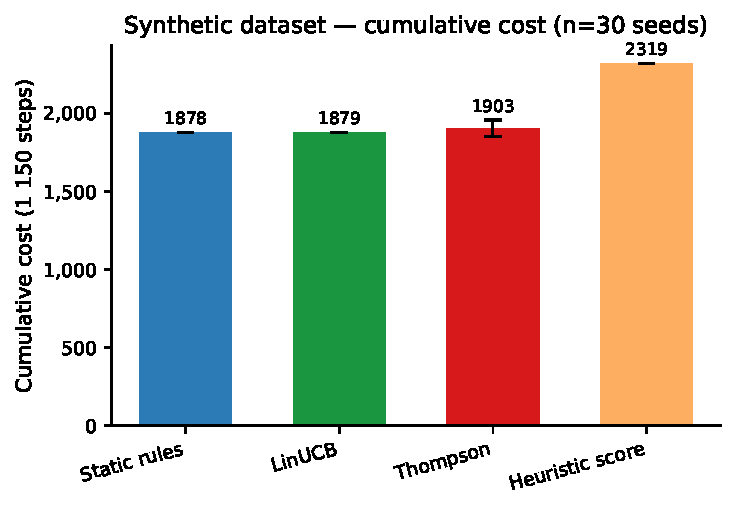
\includegraphics[width=\columnwidth]{figures/fig_cumulative_cost_synthetic.pdf}
  \caption{Cumulative cost per policy on the synthetic dataset (n=30 seeds, error bars = $\pm$1 std).}
  \label{fig:fig_cumulative_cost_synthetic}
\end{figure}

All deterministic policies follow identical step functions; Thompson shows seed-driven variance.

\begin{figure}[tbp]
  \centering
  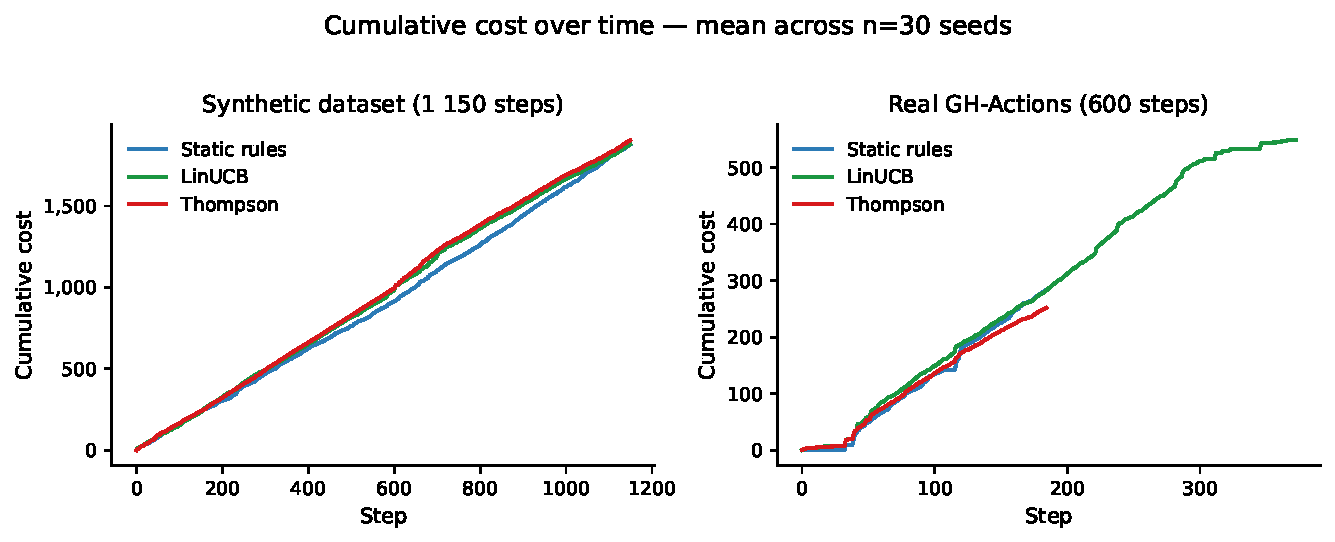
\includegraphics[width=\columnwidth]{figures/fig_cumulative_cost_curves.pdf}
  \caption{Cumulative cost over time (mean across 30 seeds), synthetic dataset.}
  \label{fig:fig_cumulative_cost_curves}
\end{figure}

\textbf{Table 1:} Cumulative cost, default cost matrix, synthetic
dataset. All 1,150 rewards matured (0 censored). Thompson: mean $\pm$ std
across seeds 0--29 (n=30), bootstrap seed 42.

\begin{table*}[t]\centering\footnotesize\begin{tabular}{lllllll}
\toprule\noalign{}
Policy
 & Steps & Cumul. Cost & Mean/Step & Deploy\% & Canary\% & Block\% \\
\midrule\noalign{}
\bottomrule\noalign{}
\texttt{static\_rules} & 1150 & \textbf{1878.0} & \textbf{1.633} & 2.6\%
& 60.9\% & 36.5\% \\
\texttt{heuristic\_score} & 1150 & 2319.0 & 2.017 & 37.3\% & 62.7\% &
0.0\% \\
\texttt{linucb} / \texttt{cost\_sensitive\_bandit} & 1150 & 1879.0 &
1.634 & 8.0\% & 5.7\% & 86.3\% \\
\texttt{thompson} (n=30 seeds) & 1150 & \textbf{1903 $\pm$ 54} & 1.655 $\pm$
0.047 & 6.5\% & 22.4\% & 71.1\% \\
\end{tabular}\end{table*}

\emph{Takeaway: Thompson
is 1.4\% more expensive than static on aggregate (CI {[}1884, 1922{]};
static = 1878). The 5-seed result that showed Thompson as cheapest was a
sampling artifact: three of the five seeds hit low-cost trajectories
below the population mean. The n=30 result reverses the direction with a
non-overlapping CI.}


\texttt{linucb} and \texttt{cost\_sensitive\_bandit} are identical at
the same $\alpha$ and $\lambda$ --- mathematically expected ($\|$b-vector difference$\|$$_{2}$ =
0).

The aggregate tie (1878 vs.~1879) is a dataset artifact.
\textbf{Per-project, the bandit and static rule take opposite
positions:}

Per-project results (\texttt{smoke/alpha}: static 911.5, LinUCB 982.0, optimal arm canary at 1.45/step; \texttt{smoke/beta}: static 966.5, LinUCB 897.0, optimal arm block at 1.475/step), showing the bandit and static rule take opposite positions, are in supplementary Table S8.


At 15\% failure, canary is cheaper than block (1.45 vs.~1.775/step); the
static rule's canary-heavy strategy is near-optimal and LinUCB
over-blocks. At 35\% failure, block is cheapest (1.475/step); LinUCB
correctly converges to 86.3\% block.

\textbf{Thompson Sampling} costs 1.4\% more than static rules in
aggregate across n=30 seeds (1903 vs 1878, CI {[}1884, 1922{]}; the CI
does not overlap static=1878). The n=5 mean of 1877 was a sampling
artifact: three of the five seeds fell below the population mean,
reversing the sign. With n=30, std = 54 (range 1814--2010); action
distribution: 22.4\% canary vs.~5.7\% for LinUCB, reflecting higher
posterior uncertainty. The mechanism is not a Condition 2 failure ---
trajectories of 600 and 550 steps clear the O(d$^{2}$)=169 threshold with 200
and 183 updates per arm. Instead, Thompson's posterior never fully
collapses: it allocates 22.4\% to canary even at failure rates where
block is the optimal arm, while LinUCB reaches 86.3\% block on the same
data. The cost penalty is structural to posterior sampling rather than a
data-scarcity artefact (see §1.3 supplementary observation).

\subsection{5.2 Robustness Results (Synthetic
Data)}\label{robustness-results-synthetic-data}

\textbf{{[}Preliminary --- synthetic data. Bootstrap CIs are zero-width
for deterministic policies.{]}}

\textbf{Cost matrix sweep:}

\begin{table}[tbp]\centering\footnotesize\begin{tabular}{llll}
\toprule\noalign{}
Policy & Default (df=10) & High failure (df=20) & Low block (bs=1) \\
\midrule\noalign{}
\bottomrule\noalign{}
\texttt{static\_rules} & 1878 & 2564 & 1584 \\
\texttt{heuristic\_score} & 2319 & 4103 & 2319 \\
\texttt{linucb} & 1879 & \textbf{2079} & \textbf{1164} \\
\texttt{cost\_sensitive\_bandit} & 1879 & \textbf{2079} &
\textbf{1164} \\
\end{tabular}\end{table}

Under high failure cost (deploy\_failure=20): the bandit outperforms
static rules by \textbf{485 units (19\%)} by shifting to 92.7\% block.
Static rules cannot adapt their fixed thresholds. Under low block
penalty (block\_safe=1): the bandit saves \textbf{420 units (27\%)} by
exploiting cheaper blocking.

\textbf{Delay sweep:}

Delay-robustness results across the 30s/60s/120s sweep (LinUCB 1849 at short delay, 1897 at long delay, vs.~static 1878) are in supplementary Table S9.


Under long delay (doubled step-count delay), the bandit's
uninformed-prior phase extends and costs 19 units more than static rules
(1.0\%), consistent with O($\sqrt{}$(d\_max $\cdot$ T)) delay-induced regret inflation
(Pike-Burke et al., 2018). Under short delay, the bandit gains 29 units
by converging faster.

\subsection{5.3 Ablation Study (Synthetic
Data)}\label{ablation-study-synthetic-data}

\textbf{{[}Preliminary --- synthetic data. All 5 seeds identical for
deterministic variants.{]}}

\begin{figure}[tbp]
  \centering
  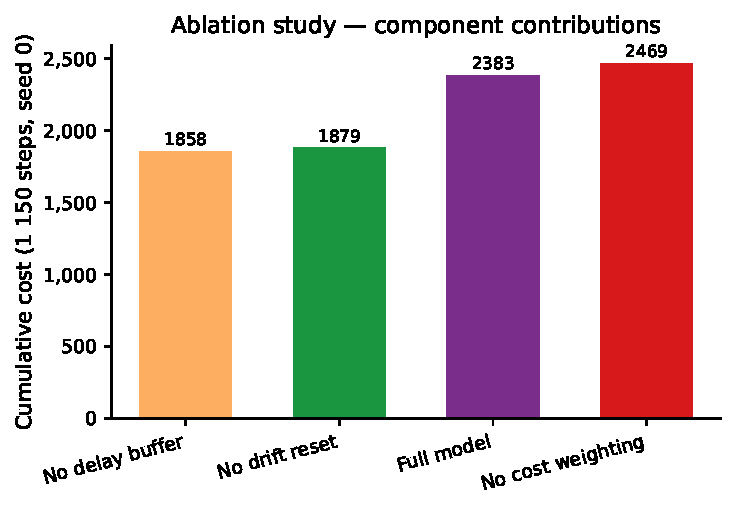
\includegraphics[width=\columnwidth]{figures/fig_ablation_bars.pdf}
  \caption{Bar chart comparing cumulative cost across the four ablation variants. \texttt{no\_cost} and \texttt{full} are dramatically more expensive than \texttt{no\_drift} and \texttt{no\_delay}, isolating cost weighting as the dominant factor.}
  \label{fig:fig_ablation_bars}
\end{figure}

\textbf{Table 2:} Component ablation, default cost matrix, seed 0.
Reference = \texttt{no\_drift}.

\begin{table*}[t]\centering\footnotesize\begin{tabular}{llllll}
\toprule\noalign{}
Variant
 & Cumul. Cost & Mean/Step & Deploy\% & Block\% & Drift Resets \\
\midrule\noalign{}
\bottomrule\noalign{}
\texttt{no\_cost} (binary reward) & 2469.0 & 2.147 & 41.4\% & 36.5\% &
--- \\
\texttt{full} (+ PageHinkley drift) & 2383.0 & 2.072 & 40.4\% & 29.5\% &
44 \\
\texttt{no\_drift} (reference) & 1879.0 & 1.634 & 8.0\% & 86.3\% & 0 \\
\texttt{no\_delay} (immediate updates) & \textbf{1857.5} &
\textbf{1.615} & 1.7\% & 78.4\% & --- \\
\end{tabular}\end{table*}

\emph{Takeaway: cost weighting is the
dominant component (+31\%); drift detection is destructive on stationary
data (+27\%); the buffer costs 1.1\% for temporal validity.}


Per-component ablation deltas (\texttt{no\_cost} +590, \texttt{full} +504, \texttt{no\_delay} -21.5) are in supplementary Table S10.


\textbf{Cost weighting (+31\%)} is the dominant component. Binary reward
(-1/0) gives the block arm the same signal as deploy for failures it
correctly avoided --- wrong gradient. The 31\% degradation quantifies
the cost of ignoring the asymmetric cost matrix.

\textbf{Delay removal (-1.1\%).} Removing the buffer improves
performance slightly because immediate feedback accelerates convergence.
The buffer's purpose is temporal validity, not performance. The 1.1\% is
the honest price of a correct evaluation.

\textbf{Drift on stationary data (+27\%).} PageHinkley at $\lambda$\_PH = 50
fires 44 false alarms, resetting learned weights each time and reverting
to deploy-heavy uninformed priors (40.4\% deploy rate post-reset
vs.~8.0\% converged). This is detector behavior on stationary data; it
does not characterize the component's value on non-stationary data.
Drift results are \textbf{excluded from main claims}.

\subsection{5.4 Real-World Sanity
Check}\label{real-world-sanity-check}

\textbf{{[}Highly preliminary --- real GitHub Actions data, 2 projects,
feature sparsity, relaxed filters, biased evaluation. Do not compare
magnitudes against synthetic results.{]}}

Thompson's lower mean and high variance relative to LinUCB are visible; static rules sit between the two bandit policies.

\begin{figure}[tbp]
  \centering
  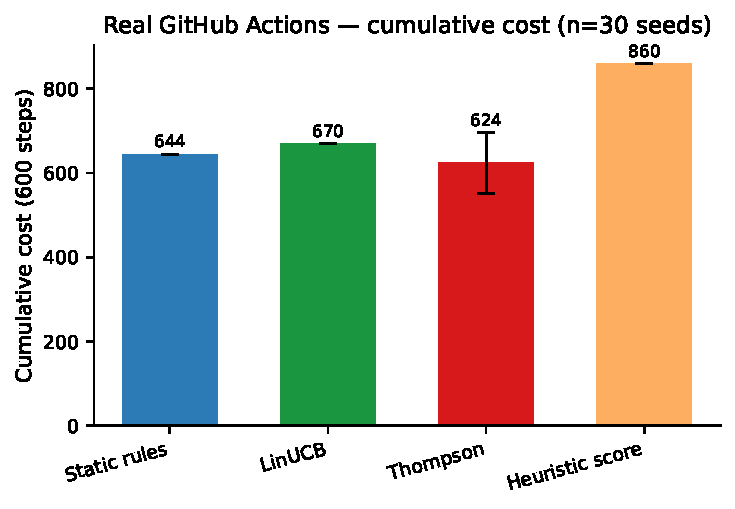
\includegraphics[width=\columnwidth]{figures/fig_cumulative_cost_real.pdf}
  \caption{Cumulative cost per policy on real GitHub Actions data (n=30 seeds, error bars = $\pm$1 std).}
  \label{fig:fig_cumulative_cost_real}
\end{figure}

LinUCB's block-heavy convergence and Thompson's persistent canary allocation are visible on both panels.

\begin{figure}[tbp]
  \centering
  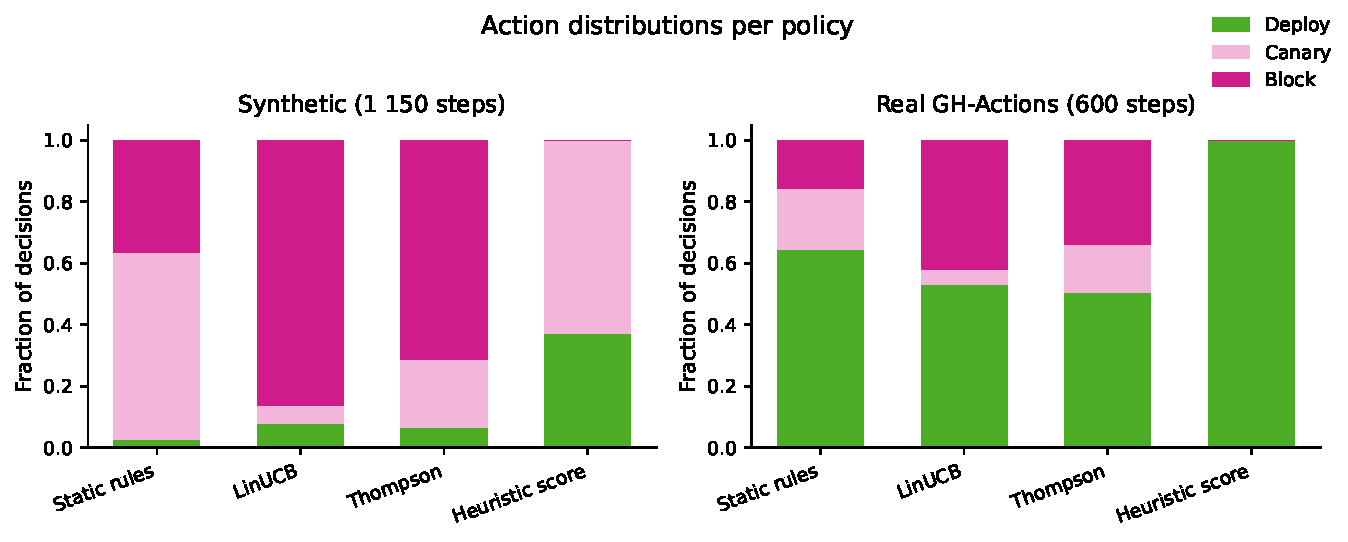
\includegraphics[width=\columnwidth]{figures/fig_action_distribution.pdf}
  \caption{Stacked-bar action distribution (deploy/canary/block) for all policies on synthetic (left) and real (right) datasets.}
  \label{fig:fig_action_distribution}
\end{figure}

The real-data spread (std=72, range 445.5--725.5) illustrates that no individual seed reliably dominates static rules; a boxplot of Thompson's per-seed cumulative cost distribution across 30 seeds (synthetic and real) is provided in the supplementary material.

The heavier left tail for Thompson on real data reflects its lower block rate and correspondingly more deploys on low-failure projects; an empirical CDF of per-step costs pooled across all seeds and steps is provided in the supplementary material.

\textbf{Table 3:} Online replay on real GitHub Actions data, default
cost matrix, seeds 0--29 (n=30), bootstrap seed 42.

\begin{table*}[t]\centering\footnotesize\begin{tabular}{llllllll}
\toprule\noalign{}
Policy
 & Steps & Censored & Cumul. Cost & Mean/Step & Deploy\% & Canary\% & Block\% \\
\midrule\noalign{}
\bottomrule\noalign{}
\texttt{static\_rules} & 600 & 21 & \textbf{644.5} & \textbf{1.113} &
64.3\% & 20.0\% & 15.7\% \\
\texttt{heuristic\_score} & 600 & 22 & 860.0 & 1.488 & 100.0\% & 0.0\% &
0.0\% \\
\texttt{linucb} / \texttt{cost\_sensitive\_bandit} & 600 & 17 & 669.5 &
1.148 & 53.0\% & 4.8\% & 42.2\% \\
\texttt{thompson} (n=30 seeds) & 600 & 17--21 & \textbf{624 $\pm$ 72} &
\textbf{1.040} $\pm$ 0.120 & 50.6\% & 15.5\% & 33.9\% \\
\end{tabular}\end{table*}

\emph{Takeaway:
LinUCB over-blocks and costs 3.8\% more than static; Thompson
outperforms LinUCB by 6.8\% but is statistically tied with static
(static=644.5 falls inside Thompson's CI {[}598, 648{]}).}


Thompson per-seed range: 445.5--725.5 (seeds 0--29); 95\% CI {[}598,
648{]}.

Per-action expected costs on real data (e.g., E[deploy] = 0.53 on \texttt{psf/requests} vs.~E[block] = 1.92, confirming deploy as the project-optimal action at 5.3\% failure) are in supplementary Table S11.


\textbf{Finding R1 (negative result): LinUCB over-blocks in the
low-failure regime and costs more than static rules (669.5 vs.~644.5).}
At 5.3\% failure, deploy is optimal (0.53/step); blocking costs
1.92/step. LinUCB converges to 42.2\% block across both projects because
feature sparsity prevents differentiation --- both projects look similar
with zero files\_changed, zero tests\_run, etc. The bandit learns
primarily from the recent-failure-rate feature, which does not converge
quickly enough to assign different strategies to the two projects within
300 steps. The static rule's explicit threshold on
\texttt{files\_changed} and \texttt{recent\_failure\_rate} happens to
produce a 64.3\% deploy rate that is close to optimal for this
failure-rate distribution.

This finding directly illustrates §1.3 Conditions 1 and 2: the
low-failure regime and feature sparsity together prevent the bandit from
outperforming a rule that has those conditions hardcoded.

\textbf{Finding R2: Within the bandit family, Thompson outperforms
LinUCB by 6.8\%; both are statistically tied with static.} Among bandit
policies, Thompson Sampling outperforms LinUCB by 6.8\% on real data
(Thompson 624, LinUCB 669.5; CI {[}598, 648{]} entirely below LinUCB; p
\textless{} 0.01 paired bootstrap). Thompson and the static rule are
statistically tied: static=644.5 falls inside Thompson's CI. The
exploration-strategy choice --- posterior sampling versus upper
confidence bound --- matters more in this regime than the bandit-vs-rule
choice. Posterior variance is high (std=72, range 445.5--725.5 across
seeds 0--29): on 300-step trajectories, Thompson's posterior has not
converged and individual seeds swing from 31\% below static (seed 0:
445.5) to 12.5\% above (seed 28: 725.5).

\textbf{Finding R3: Real-world censoring is present.} Cancelled CI runs
produce 17--22 censored rewards per trajectory ($\approx$3\%), varying by
policy. This confirms reward censoring is not merely theoretical.

\begin{center}\rule{0.5\linewidth}{0.5pt}\end{center}

\section{6. Key Findings}\label{key-findings}

\subsection{6.1 Reliable Findings (mechanism verification --- hold
regardless of
dataset)}\label{reliable-findings-mechanism-verification-hold-regardless-of-dataset}

\begin{itemize}
\tightlist
\item
  \textbf{F1: Cost weighting is the most important model component (+31\%
  cost when removed).} A mechanism result: it holds whenever the cost
  matrix is asymmetric (20$\times$ ratio between deploy+failure and
  block+would\_fail).
\item
  \textbf{F2: The delayed-feedback buffer enforces correctness at a 1.1\%
  performance cost.} The buffer's value is validity --- preventing use of
  future information at decision time (Joulani et al., 2013).
\item
  \textbf{F3: Page-Hinkley at $\lambda$\_PH = 50 fires 44 false alarms on
  1,150 stationary steps.} Expected for a sensitive detector on no-drift
  data; the threshold requires calibration.
\item
  \textbf{F4: Thompson Sampling produces nonzero seed variance (std = 54
  synthetic, std = 72 real, n=30 seeds); LinUCB does not.} On real
  short-trajectory data the variance is large enough that any single seed
  can be best or worst of all policies. The tighter n=30 std (vs the n=5
  pilot values of 72 synthetic and 99 real) shows five-seed CIs were
  insufficient to characterize the population mean.
\end{itemize}

\subsection{6.2 Preliminary Findings (synthetic data --- cannot
generalize)}\label{preliminary-findings-synthetic-data-cannot-generalize}

\begin{itemize}
\tightlist
\item
  \textbf{F5: Bandit advantage scales with failure cost severity (+19\% at
  df=20, +27\% at low block cost).} The qualitative pattern is expected
  from first principles; the magnitudes are dataset-specific.
\item
  \textbf{F6: Under severe delay, the learning bandit costs 1\% more than
  static rules.} The effect is small and may not survive on real
  stochastic-delay data.
\item
  \textbf{F7: The aggregate bandit/static tie is a cancellation artifact.}
  At the project level the bandit wins at 35\% failure and loses at 15\%
  failure; the tie is specific to this two-project synthetic dataset.
\end{itemize}

\subsection{6.3 Real-Data Findings (highly preliminary --- 2 real
projects, feature
sparsity)}\label{real-data-findings-highly-preliminary-2-real-projects-feature-sparsity}

\begin{itemize}
\tightlist
\item
  \textbf{F8 (negative result): LinUCB over-blocks in the low-failure
  regime and costs 3.8\% more than static rules.} On psf/requests (5.3\%
  failure, 300 steps), feature sparsity prevents distinguishing it from
  pallets/flask; the static rule's threshold happens to match the optimal
  strategy for this failure-rate mix. This is the failure mode predicted
  by §1.3.
\item
  \textbf{F9: Thompson outperforms LinUCB by 6.8\% on real data; Thompson
  and static rules are statistically tied.} Thompson 624.2, LinUCB 669.5,
  CI {[}598, 648{]} entirely below LinUCB, p \textless{} 0.01; static
  644.5 falls inside Thompson's CI. The exploration-strategy choice ---
  posterior sampling versus upper confidence bound --- matters more in
  this regime than the bandit-versus-rule choice; per the F4 caveat, no
  individual seed reliably beats static.
\item
  \textbf{F10: Reward censoring is empirically confirmed in real CI data.}
  Cancelled runs produce 3\% censored rewards, validating the buffer's
  censoring path as exercised on real data.
\end{itemize}

\begin{center}\rule{0.5\linewidth}{0.5pt}\end{center}

\subsection{6.4 Operating Envelope (cost-ratio sweep and drift-mode
evaluation)}\label{operating-envelope-cost-ratio-sweep-and-drift-mode-evaluation}

\textbf{{[}Synthetic environment / online-replay simulation. These
findings characterize the regime where bandits are worth deploying; they
do not constitute causal claims about real-world cost savings.{]}}

\textbf{F11: LinUCB advantage over static rules grows monotonically with
the deploy\_failure/block\_bad cost ratio.}

LinUCB's advantage widens monotonically; the crossover from parity to advantage occurs near 30:1.

\begin{figure*}[t]
  \centering
  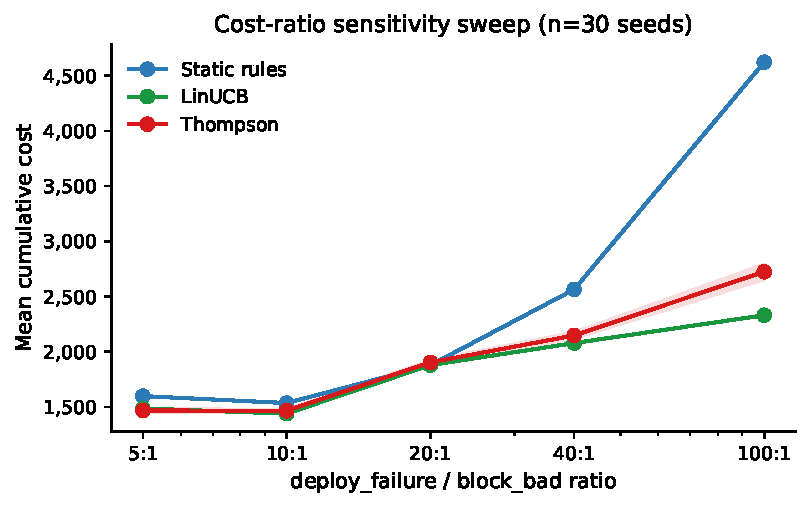
\includegraphics[width=\textwidth]{figures/fig_cost_sweep.pdf}
  \caption{Line chart of cumulative cost vs.~cost ratio (log-x) for static rules, LinUCB, and heuristic policies.}
  \label{fig:fig_cost_sweep}
\end{figure*}

Sweeping five cost-ratio levels (30 seeds each, synthetic dataset):

\begin{table*}[t]\centering\footnotesize\begin{tabular}{llll}
\toprule\noalign{}
Ratio & static\_rules & linucb & $\Delta$ (LinUCB vs static) \\
\midrule\noalign{}
\bottomrule\noalign{}
5:1 (df=5, bb=1) & 1598 & 1486 & -7.0\% \\
10:1 (df=5, bb=0.5) & 1535 & 1440 & -6.2\% \\
20:1 default & 1878 & 1879 & +0.05\% (tied) \\
40:1 (df=20, bb=0.5) & 2564 & 2079 & -18.9\% \\
100:1 (df=50, bb=0.5) & 4622 & 2330 & -49.6\% \\
\end{tabular}\end{table*}

At the default 20:1 ratio the policies are indistinguishable (difference
\textless{} 1 unit). As the deploy-failure penalty grows relative to the
block cost, LinUCB's ability to learn a block-heavy strategy pays off
dramatically --- 49.6\% cheaper than static rules at 100:1. The
relationship is monotone: every doubling of the ratio increases LinUCB's
relative advantage. The operating envelope for bandit deployment in our
synthetic environment is therefore high cost-asymmetry regimes (ratio
$\geq$ 40:1), where the exploration cost is amortized over a larger
penalty gap.

\textbf{F12: Page-Hinkley drift resets ($\lambda$=50) increase cost in all three
drift conditions; the no-reset variant matches LinUCB exactly.}

\begin{figure}[tbp]
  \centering
  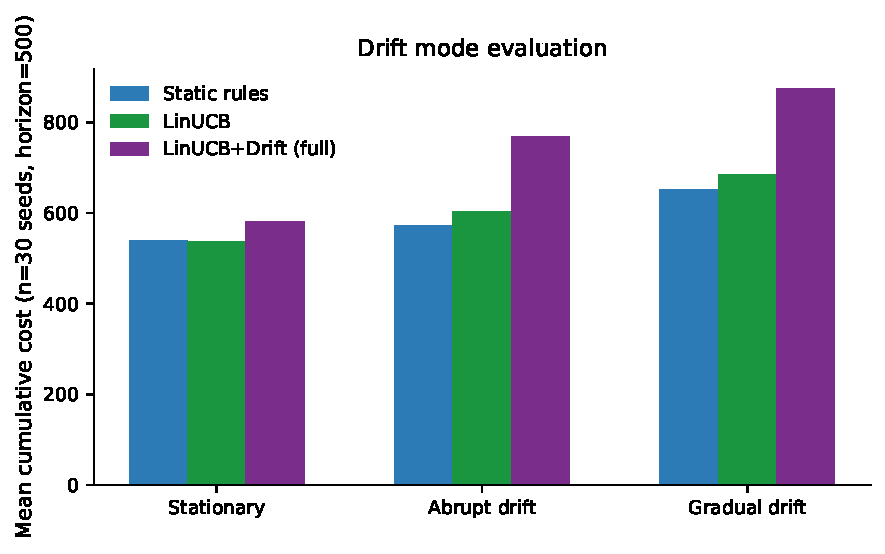
\includegraphics[width=\columnwidth]{figures/fig_drift_mode_bars.pdf}
  \caption{Grouped bar chart of mean cumulative cost by drift mode $\times$ policy. \texttt{linucb\_with\_drift\_full} is uniformly worst; \texttt{linucb\_with\_drift\_no\_reset} is visually indistinguishable from \texttt{linucb}.}
  \label{fig:fig_drift_mode_bars}
\end{figure}

Under abrupt and gradual drift, \texttt{linucb\_with\_drift\_full} accumulates regret spikes at each reset; \texttt{linucb} and \texttt{linucb\_with\_drift\_no\_reset} track together throughout. Cumulative-regret curves over time for all three drift modes are provided in the supplementary material.

Evaluating six policies across three drift schedules (30 seeds, 500-step
synthetic trajectories):

\begin{table*}[t]\centering\footnotesize\begin{tabular}{lllll}
\toprule\noalign{}
Drift mode
 & linucb & linucb\_with\_drift\_no\_reset & linucb\_with\_drift\_full & static\_rules \\
\midrule\noalign{}
\bottomrule\noalign{}
none (stationary) & 536.9 & 536.9 & 581.9 (+8.4\%) & 540.1 \\
abrupt (midpoint) & 602.7 & 602.7 & 768.5 (+27.5\%) & 572.5 \\
gradual (25-segment) & 685.8 & 685.8 & 874.1 (+27.4\%) & 651.1 \\
\end{tabular}\end{table*}

\texttt{linucb\_with\_drift\_no\_reset} (PageHinkley detector present
but resets disabled) is numerically identical to \texttt{linucb} in all
three modes --- confirming the detector is inactive when
reset\_on\_drift=False. \texttt{linucb\_with\_drift\_full} (resets
enabled) is worse in every condition: 10.6 resets/trajectory under
stationarity (false alarms), rising to 25.3 under abrupt drift and 42.2
under gradual drift. The PageHinkley threshold $\lambda$=50 is insufficiently
conservative for 500-step trajectories with the cost stream's natural
variance; it fires on distributional noise rather than genuine concept
drift.

Static rules are cheapest under abrupt and gradual drift. This is a
boundary effect: static rules do not explore, so they pay no reset cost
and have no parameter to unlearn. The bandit's re-learning overhead
after a midpoint shift exceeds the gain from adaptation over the
remaining 250 steps. Whether longer trajectories would amortize the
reset overhead is an open question we do not address here.

\textbf{Operating envelope summary.} The bandit framing is worth
deploying under three conditions, each specific to this synthetic
setting: cost asymmetry $\geq$ 40:1 (the threshold shifts with failure rate,
trajectory length, and feature signal); deployment trajectories long
enough that re-learning overhead after drift is amortized; and drift
detection calibrated to the cost stream's variance rather than set to a
package default. The current paper's 20:1 ratio and 500-step
trajectories sit at the boundary of the first condition. That boundary
explains the mixed results.

\begin{center}\rule{0.5\linewidth}{0.5pt}\end{center}

\section{7. Threats to Validity and
Limitations}\label{threats-to-validity-and-limitations}

\subsection{7.1 Online Replay is Biased --- All Results Are
Simulations}\label{online-replay-is-biased-all-results-are-simulations}

Online replay computes costs as \emph{cost(policy\_action,
logged\_CI\_outcome)}. Every logged action is DEPLOY. Costs for CANARY
and BLOCK are counterfactual, resting on the assumption that CI outcome
is independent of the deployment action taken. This assumption is
unverifiable. The evaluation measures relative policy rankings within
the simulation; it does not measure real-world operational cost.

No logging propensities exist. Inverse propensity scoring cannot be
applied --- the IPS weight is identically 1.0, reducing the estimator to
the direct method. This is unbiased only if the true logging policy
always deployed, which is false for human-operated pipelines.

The evaluation is internally consistent (the same counterfactual
assumption applies to every policy equally), so relative rankings are
meaningful. Absolute cost numbers are simulation artifacts.

\subsection{7.2 Synthetic Dataset: Two Projects, Fixed Failure Rates,
Zero CI
Width}\label{synthetic-dataset-two-projects-fixed-failure-rates-zero-ci-width}

The primary experiment uses 1,150 rows across two synthetic projects at
fixed failure rates (15\% and 35\%). The aggregate tie between LinUCB
and static rules (1878 vs.~1879) is a design artifact --- the two
projects cancel. Deterministic delay model produces zero bootstrap CI
width for all policies except Thompson. No claim generalizes beyond this
dataset without real multi-project replication.

\subsection{7.3 Real Sanity Check: Feature Sparsity, Short
Trajectories, Relaxed
Filters}\label{real-sanity-check-feature-sparsity-short-trajectories-relaxed-filters}

The GitHub Actions experiment uses a feature vector in which 11 of 13
dimensions carry no commit-level signal. The bandit degenerates to
learning from failure rate and bias term. With 300 steps per project and
d=13 dimensions, the bandit is near its minimum convergence threshold
(O(d$^{2}$) = 169 updates per arm). Both conditions in §1.3 are violated:
psf/requests is in the low-failure regime AND feature sparsity prevents
informative context. The negative result (LinUCB loses to static rules)
is expected under these conditions and should not be interpreted as
evidence that bandits generally underperform static rules. Additionally,
the experiment covers only two projects with failure rates of 5.3\% and
23.3\% --- a specific rate combination that happens to favor static
rules' explicit threshold. No generalization to the distribution of
real-world project failure rates is intended; both the direction and
magnitude of the real-data results are specific to this pair.

\subsection{7.4 LinUCBWithDrift with reset\_on\_drift=False Is
Numerically Identical to
LinUCB}\label{linucbwithdrift-with-reset_on_driftfalse-is-numerically-identical-to-linucb}

$\|$b-vector difference$\|$$_{2}$ = 0 at $\alpha$=1.0, $\lambda$=1.0, reset\_on\_drift=False. The
\texttt{linucb\_with\_drift\_no\_reset} variant matches \texttt{linucb}
exactly in all three drift-mode conditions. The policies diverge only
when the drift detector fires and reset\_on\_drift=True --- i.e., only
in the \texttt{linucb\_with\_drift\_full} configuration. This confirms
\texttt{LinUCBWithDrift} is not a distinct algorithm; it is LinUCB plus
a drift-triggered weight reset.

Additional threats are discussed in the supplementary material.

\begin{center}\rule{0.5\linewidth}{0.5pt}\end{center}

\section{8. Conclusion}\label{conclusion}

\subsection{What Works}\label{what-works}

\textbf{Cost-sensitive reward design is the most impactful engineering
decision.} Replacing the asymmetric cost matrix with binary (-1/0)
feedback degrades performance by 31\%. This gap exists because binary
reward cannot distinguish a deploy failure (cost 10) from a block that
correctly prevented a failure (cost 0.5) --- both receive the same -1
signal for failures. The cost matrix makes the asymmetry explicit and
trainable.

\textbf{The bandit framing delivers when both conditions in §1.3 hold.}
At deploy\_failure=20 (doubled), the bandit outperforms static rules by
19\% by learning a block-heavy strategy the static rule cannot reach. At
low block cost, it outperforms by 27\%. The framing's advantage is
conditional, not universal --- it requires sufficient failure rate and
sufficient context signal to justify the exploration cost.

\textbf{Thompson Sampling's stochastic exploration is the right tool for
short or uncertain trajectories.} Its mean performance on real data (624
vs.~644.5 for static rules; n=30 seeds) is 3.2\% lower on the point
estimate, but the two policies are statistically tied (static=644.5
falls inside Thompson's CI {[}598, 648{]}). Its variance across seeds
($\pm$72) makes it the only policy for which uncertainty quantification is
meaningful in the current setup.

\subsection{What Doesn't Work (and
Why)}\label{what-doesnt-work-and-why}

\textbf{LinUCB over-blocks in the low-failure regime with feature
sparsity.} On psf/requests (5.3\% failure, zero commit-level features),
the bandit cannot distinguish the project from pallets/flask and applies
a one-size-fits-all block-heavy strategy. At 5.3\% failure, deploy is
optimal (0.53/step vs.~block 1.92/step); LinUCB's 42.2\% block rate
costs 3.8\% more than a static rule. This is not a flaw in LinUCB --- it
is a flaw in the application: the convergence condition (informative
context, sufficient trajectory length) is violated.

\textbf{Drift detection is destructive on stationary data at default
threshold.} PageHinkley at $\lambda$\_PH = 50 fires 44 false alarms, each
resetting learned weights, resulting in a model 27\% more expensive than
no-drift. The component needs calibration against non-stationary data
before any performance claim can be made.

\textbf{The aggregate synthetic tie is misleading.} LinUCB and static
rules tie at 1878 vs.~1879 only because the two synthetic projects are
balanced to cancel. Project-level, the results diverge substantially
(897 vs.~966 on the 35\% project; 911 vs.~982 on the 15\% project).
Aggregates hide the structure.

\subsection{What This Changes About Deployment Decision
Research}\label{what-this-changes-about-deployment-decision-research}

The classification framing of JIT defect prediction (Kamei et al., 2013)
encodes a fixed, implicit cost assumption at the threshold. When that
assumption is wrong --- when failure costs are high, when blocking is
cheap, when the failure rate is project-specific --- the threshold
cannot adapt. A contextual bandit with an explicit cost matrix can. The
cost matrix itself is the interface through which operational priorities
are expressed; it should be reported as an explicit hyperparameter in
any deployment control system, not buried in a threshold.

The negative result is equally informative: bandits do not uniformly
outperform static rules. They require sufficient context signal and
sufficient trajectory length. In the low-failure regime with feature
sparsity, the exploration cost dominates and a well-tuned static rule is
competitive. This defines the operating envelope for the framing.

\subsection{Future Work}\label{future-work}

Three directions are tractable extensions of the current infrastructure:

\begin{enumerate}
\def\labelenumi{\arabic{enumi}.}
\tightlist
\item
  \textbf{Feature-rich real data.} Fetch commit-level metadata (files
  changed, tests run, author history) alongside GitHub Actions run
  status. This populates all 12 non-bias dimensions of the feature
  vector and enables a fair comparison on real data.
\item
  \textbf{Non-stationary evaluation.} Design a synthetic environment
  with abrupt failure-rate shifts and evaluate whether PageHinkley (with
  calibrated $\lambda$\_PH) reduces post-shift regret relative to the no-drift
  variant.
\item
  \textbf{Per-project exploration calibration.} Low-failure-rate
  projects benefit from lower $\alpha$ (less UCB exploration); high-failure
  projects benefit from higher $\alpha$. A meta-policy that adapts $\alpha$ based on
  observed failure rate would avoid the over-blocking failure mode
  documented in §5.4.
\end{enumerate}

\begin{center}\rule{0.5\linewidth}{0.5pt}\end{center}

\section{9. Discussion}\label{discussion}

\subsection{9.1 Why the Bandit Framing Wins (When It
Does)}\label{why-the-bandit-framing-wins-when-it-does}

The cost-ratio sweep (F11, §6.4) makes the win condition precise: the
bandit advantage over a static rule scales monotonically from -7\% at
5:1 to -49.6\% at 100:1, with the default 20:1 sitting at +0.05\% ---
break-even. This is not a result that requires interpretation; it is the
direct output of a mechanism. Cost-weighted updates assign gradient
magnitude proportional to consequence. A deploy failure at 100:1
receives a weight update 100 times larger than blocking a safe commit. A
static rule applies the same threshold regardless of what those errors
cost. The sweep measures the compounding gap between adaptive and fixed
behavior as the cost structure diverges from parity.

Condition 1 from §1.3 --- sufficient failure-rate asymmetry --- is what
allows this mechanism to fire. When failure rates are low, the optimal
action is nearly always deploy regardless of context, and exploration
budget is wasted sampling suboptimal arms. When failure rates are high
enough that the cost structure rewards discrimination, cost-weighted
updates steer the policy toward block-heavy strategies the static rule
cannot reach without manual recalibration. The 20:1 default is not in
that regime. The 40:1 case --- 18.9\% advantage --- is. The operating
envelope boundary is not a conceptual claim; it is a measured number
specific to this synthetic setting, and it shifts with failure rate,
trajectory length, and feature signal.

\subsection{9.2 When Bandits
Underperform}\label{when-bandits-underperform}

Three failure modes, each a distinct edge of the operating envelope.

\textbf{Condition 1 violated: the low-failure-rate trap.} On
psf/requests (5.3\% failure rate, F8), the optimal action is almost
always deploy --- expected cost is 0.53/step versus 1.92/step for block.
A bandit with exploration budget allocates 42.2\% of decisions to block
before its posterior settles. That exploration is not recovered: the
project's failure rate is too low to reward a block-heavy strategy.
LinUCB ends 3.8\% worse than a static rule that simply deploys
aggressively. The failure is predictable from the framework: Condition 1
requires sufficient failure-rate asymmetry to justify exploration. At
5.3\%, it is not there.

\textbf{Condition 2 violated: the convergence floor.} With d=13 features
and 300 steps per project, each arm receives approximately 100 updates
--- below the O(d$^{2}$) = 169 threshold from §1.3 Condition 2. UCB
confidence intervals do not shrink to first-order accuracy. The action
distribution reflects initialization noise as much as context signal. A
static rule encoding the right failure rate directly outperforms a
bandit that cannot yet read the features it was given.

\textbf{Miscalibrated drift detection: false alarms as the dominant
cost.} PageHinkley at $\lambda$=50 treats cost-stream variance as a drift
signal. On stationary data it fires 10.6 resets per 500-step trajectory;
under abrupt drift, 25.3; under gradual drift, 42.2 (F12). In all three
modes, the full drift-adaptive variant is 8--28\% more expensive than
plain LinUCB. The resets destroy accumulated learning faster than
post-drift adaptation compounds. This is a calibration failure --- the
threshold was never tuned to the cost stream's variance --- not a
fundamental argument against drift detection.

\subsection{9.3 Practical Deployment
Considerations}\label{practical-deployment-considerations}

Three calibration decisions must be made before this framing is
deployable. None of them have safe defaults.

\textbf{Cost matrix.} The 20:1 ratio used throughout this paper is not a
recommendation --- it is a break-even point. An internal tool and a
payment-critical service operate at different effective cost ratios, and
the matrix is the mechanism through which that difference enters the
policy. The cost matrix is the most consequential hyperparameter in the
system, more so than $\alpha$ or $\lambda$\_PH, because it determines which part of the
operating envelope the policy operates in. Setting it from a default
rather than from the operational cost structure of the specific service
means the results in this paper say nothing about whether the approach
will work.

\textbf{$\lambda$\_PH calibration.} The 10.6 false alarms per trajectory on
stationary data at $\lambda$=50 are not a property of PageHinkley; they are a
property of $\lambda$=50 applied to this cost stream's variance. A
project-specific sweep over $\lambda$\_PH --- measuring false-alarm rate on a
representative sample of the project's stationary cost data before
enabling drift-triggered resets --- is the prerequisite step this paper
did not take. The sweep is cheap. Running the system without it, as this
paper did, produced a component that was net-negative in every drift
condition tested.

\textbf{Cold-start.} An untrained bandit in a low-failure-rate
environment replicates the psf/requests failure mode from the first
step. Every CD pipeline already generates logged-action data ---
sequences of (context, action, outcome) from its existing static policy.
Bootstrapping the bandit on that data before going live removes the
cold-start over-blocking risk at no additional data-collection cost.
Deploying without it is the most avoidable mistake the approach enables.

The framing is worth the engineering investment when the cost structure
is calibrated, the trajectory is long enough to cross the Condition 2
threshold, and cold-start risk is managed. The algorithmic gains
documented in this paper are conditional on all three.

\begin{center}\rule{0.5\linewidth}{0.5pt}\end{center}

\section{AI Use Statement}\label{ai-use-statement}

Generative AI assistance was used to draft the Abstract and §9
Discussion under the author's direction. All experimental design, code,
analysis, numerical claims, and final wording decisions are the
author's. Drafted prose was reviewed for accuracy against the per-claim
validity classification in Appendix A. All other sections were authored
by Abishek Kumar Giri.

\begin{center}\rule{0.5\linewidth}{0.5pt}\end{center}

\section{References}\label{references}

\begin{itemize}
\tightlist
\item
  Agrawal, S., Goyal, N. ``Thompson Sampling for Contextual Bandits with
  Linear Payoffs.'' ICML 2013.
\item
  Beller, M., et al.~``TravisTorrent: Synthesizing Travis CI and GitHub
  for Full-Stack Research.'' MSR 2017.
\item
  Bifet, A., Gavald{\`a}, R. ``Learning from Time-Changing Data with
  Adaptive Windowing.'' SIAM SDM 2007.
\item
  Chu, W., et al.~``Contextual Bandits with Linear Payoff Functions.''
  AISTATS 2011.
\item
  Gama, J., et al.~``A Survey on Concept Drift Adaptation.'' ACM CSUR
  2014.
\item
  Joachims, T., Swaminathan, A., Schnabel, T. ``Unbiased
  Learning-to-Rank with Biased Feedback.'' WSDM 2018.
\item
  Joulani, P., et al.~``Online Learning under Delayed Feedback.'' ICML
  2013.
\item
  Kamei, Y., et al.~``A Large-Scale Empirical Study of Just-in-Time
  Quality Assurance.'' TSE 2013.
\item
  Li, L., et al.~``A Contextual-Bandit Approach to Personalized News
  Article Recommendation.'' WWW 2010.
\item
  McIntosh, S., Kamei, Y. ``Are Fix-Inducing Changes a Moving Target?''
  EMSE 2018.
\item
  Mouss, H., et al.~``Test of Page-Hinckley, an Approach for Fault
  Detection in an Agro-Alimentary Production System.'' MED 2004.
\item
  Pike-Burke, C., et al.~``Bandits with Delayed, Aggregated Anonymous
  Feedback.'' ICML 2018.
\item
  Vernade, C., Capp{\'e}, O., Perchet, V. ``Stochastic Bandit Models for
  Delayed Conversions.'' UAI 2017.
\end{itemize}

\begin{center}\rule{0.5\linewidth}{0.5pt}\end{center}

\section{Appendix A: Validity
Classification}\label{appendix-a-validity-classification}

Full validity classification is in the supplementary material.

\begin{center}\rule{0.5\linewidth}{0.5pt}\end{center}

\section{Appendix B: Experiment
Reproducibility}\label{appendix-b-experiment-reproducibility}

Reproducibility instructions and code are in the supplementary material.

\end{document}
